% !TeX program = xelatex
\documentclass[10pt]{beamer}

\usetheme{metropolis}

\usepackage{pgfplots}
\usepgfplotslibrary{fillbetween}
\usepackage{pgfopts}
\usepackage{amsmath}
\usepackage{structuralanalysis}
\usepackage{tikz}
\usepackage{tikz-3dplot}
\usepackage{chngcntr}
\usepackage{wasysym}
\usepackage{mathtools}
\usepackage{alphalph}
\usepackage{xcolor}
\usepackage[showdow=false, en-US]{datetime2}
\usepackage{hyperref}

\newcommand{\highlight}[1]{%
	\colorbox{red!50}{$\displaystyle#1$}}

\setcounter{lecture}{18}
\counterwithin{equation}{lecture}
\makeatletter
\def\user@resume{resume}
\def\user@intermezzo{intermezzo}
%
\newcounter{previousequation}
\newcounter{lastsubequation}
\newcounter{savedparentequation}
\setcounter{savedparentequation}{1}
% 
\renewenvironment{subequations}[1][]{%
	\def\user@decides{#1}%
	\setcounter{previousequation}{\value{equation}}%
	\ifx\user@decides\user@resume 
	\setcounter{equation}{\value{savedparentequation}}%
	\else  
	\ifx\user@decides\user@intermezzo
	\refstepcounter{equation}%
	\else
	\setcounter{lastsubequation}{0}%
	\refstepcounter{equation}%
	\fi\fi
	\protected@edef\theHparentequation{%
		\@ifundefined {theHequation}\theequation \theHequation}%
	\protected@edef\theparentequation{\theequation}%
	\setcounter{parentequation}{\value{equation}}%
	\ifx\user@decides\user@resume 
	\setcounter{equation}{\value{lastsubequation}}%
	\else
	\setcounter{equation}{0}%
	\fi
	\def\theequation  {\theparentequation  \alph{equation}}%
	\def\theHequation {\theHparentequation \alph{equation}}%
	\ignorespaces
}{%
%  \arabic{equation};\arabic{savedparentequation};\arabic{lastsubequation}
\ifx\user@decides\user@resume
\setcounter{lastsubequation}{\value{equation}}%
\setcounter{equation}{\value{previousequation}}%
\else
\ifx\user@decides\user@intermezzo
\setcounter{equation}{\value{parentequation}}%
\else
\setcounter{lastsubequation}{\value{equation}}%
\setcounter{savedparentequation}{\value{parentequation}}%
\setcounter{equation}{\value{parentequation}}%
\fi\fi
%  \arabic{equation};\arabic{savedparentequation};\arabic{lastsubequation}
\ignorespacesafterend
}
\makeatother
\title{AE 737 - Mechanics of Damage Tolerance}
\subtitle{Lecture \arabic{lecture}}
\date{Last Updated: \today\ at \DTMcurrenttime}
\author{Dr. Nicholas Smith}
\institute{Wichita State University, Department of Aerospace Engineering}
% \titlegraphic{\hfill\includegraphics[height=1.5cm]{logo/logo}}

\begin{document}

\maketitle
\begin{frame}{schedule}
	\begin{itemize}
		\item 31 Mar - Strain based fatigue, project abstract due
		\item 5 Apr - Crack Growth, Homework 7 due, Homework 8 assigned
		\item 7 Apr - Crack Growth, Stress Spectrum
		\item 12 Apr - Retardation, Boeing Commercial Method
		\item 14 Apr - Exam Review, Homework 8 Due
		\item 19 Apr - Exam 2
		\item 21 Apr - Exam Solutions, Damage Tolerance
%		\item 26 Apr - Damage Tolerance, AFGROW
%		\item 28 Apr - AFGROW, Finite Elements
%		\item 3 May - Finite Elements
%		\item 5 May - Non-Destructive Testing, Composites, Final Project Due May 10
	\end{itemize}
\end{frame}

\begin{frame}
  \frametitle{outline}
  \setbeamertemplate{section in toc}[sections numbered]
  \tableofcontents[hideallsubsections]
\end{frame}

\section{strain based fatigue}

\begin{frame}{strain based fatigue}
	\begin{itemize}[<+->]
		\item The strain based fatigue method uses local stresses and strains (instead of global, nominal values)
		\item The strain-based method gives greater detail, and validity at lower cycles
		\item It is still valid for high cycle fatigue
		\item Does not include crack growth analysis or fracture mechanics
	\end{itemize}
\end{frame}

\begin{frame}{strain life curve}
	\begin{itemize}[<+->]
		\item Similar to the S-N curves in stress-based fatigue analysis, we can plot the cyclic strain amplitude vs. number of cycles to failure
		\item This is most commonly done using axial test machines (instead of rotating bending tests)
		\item The test is run in strain control (not load control)
		\item Generally plotted on log-log scale
	\end{itemize}
\end{frame}

\begin{frame}{plastic and elastic strain}
	\begin{itemize}[<+->]
		\item We can separate the total strain into elastic and plastic components
		\item[] \begin{equation}
		\epsilon_a = \epsilon_{ea} + \epsilon_{pa}
		\end{equation}
	\end{itemize}
\end{frame}

\begin{frame}{plastic strain}
	\begin{figure}
	\centering
	\includegraphics[width=0.7\linewidth]{"../Figures/plastic_strain"}
	\label{fig:plasticstrain}
	\end{figure}
\end{frame}

\begin{frame}{hysteresis loops}
	\begin{figure}
	\centering
	\includegraphics[width=0.7\linewidth]{"../Figures/hysteresis_loops"}
	\label{fig:hysteresisloops}
\end{figure}
\end{frame}

\begin{frame}{cyclic stress strain curve}
	\begin{itemize}[<+->]
		\item While strain-life data will generally just report $\epsilon_a$ and $\epsilon_{pa}$, some will also tabulate a form for the cyclic stress-strain curve
		\item[] \begin{equation}
		\epsilon_a = \frac{\sigma_a}{E} + \left(\frac{\sigma_a}{H^\prime}\right)^{\frac{1}{n^\prime}}
		\end{equation}
	\end{itemize}
\end{frame}

\begin{frame}{plastic and elastic strain}
	\begin{itemize}[<+->]
		\item On strain life curves, the strain is often plotted three times per each experiment
		\item Once for total strain, once for plastic strain, and once for elastic strain
		\item Since plastic strain and elastic strain vary by the number of cycles, a hysteresis loop from half the fatigue life is generally used
		\item This is considered representative of stable behavior
	\end{itemize}
\end{frame}

\begin{frame}{experimental data}
	\begin{figure}
	\centering
	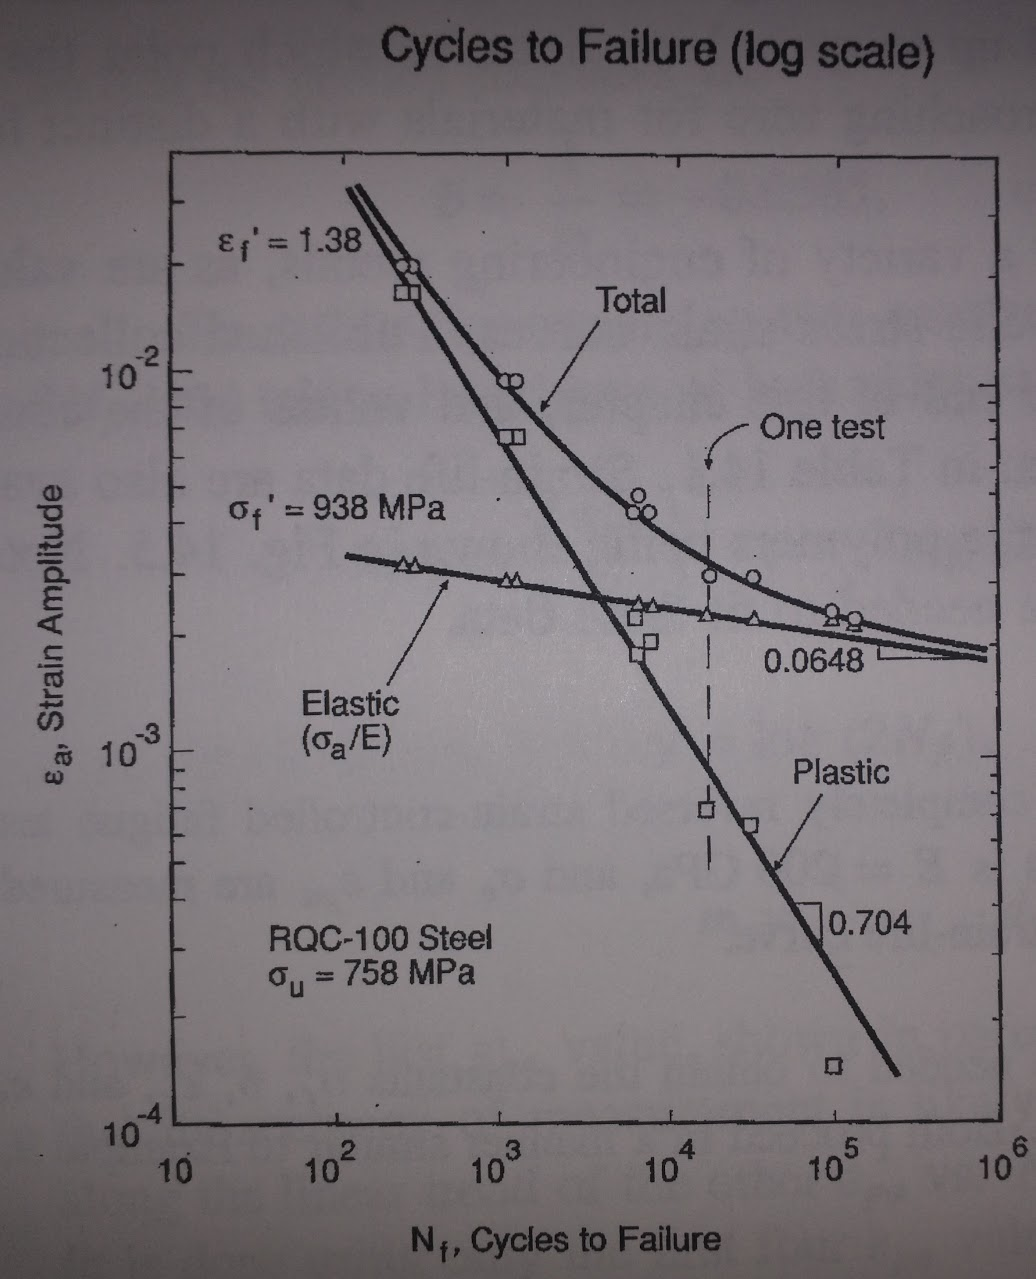
\includegraphics[width=0.5\linewidth]{../Figures/strain-life}
	\label{fig:strain-life}
	\end{figure}
\end{frame}

\begin{frame}{trends}
	\begin{figure}
	\centering
	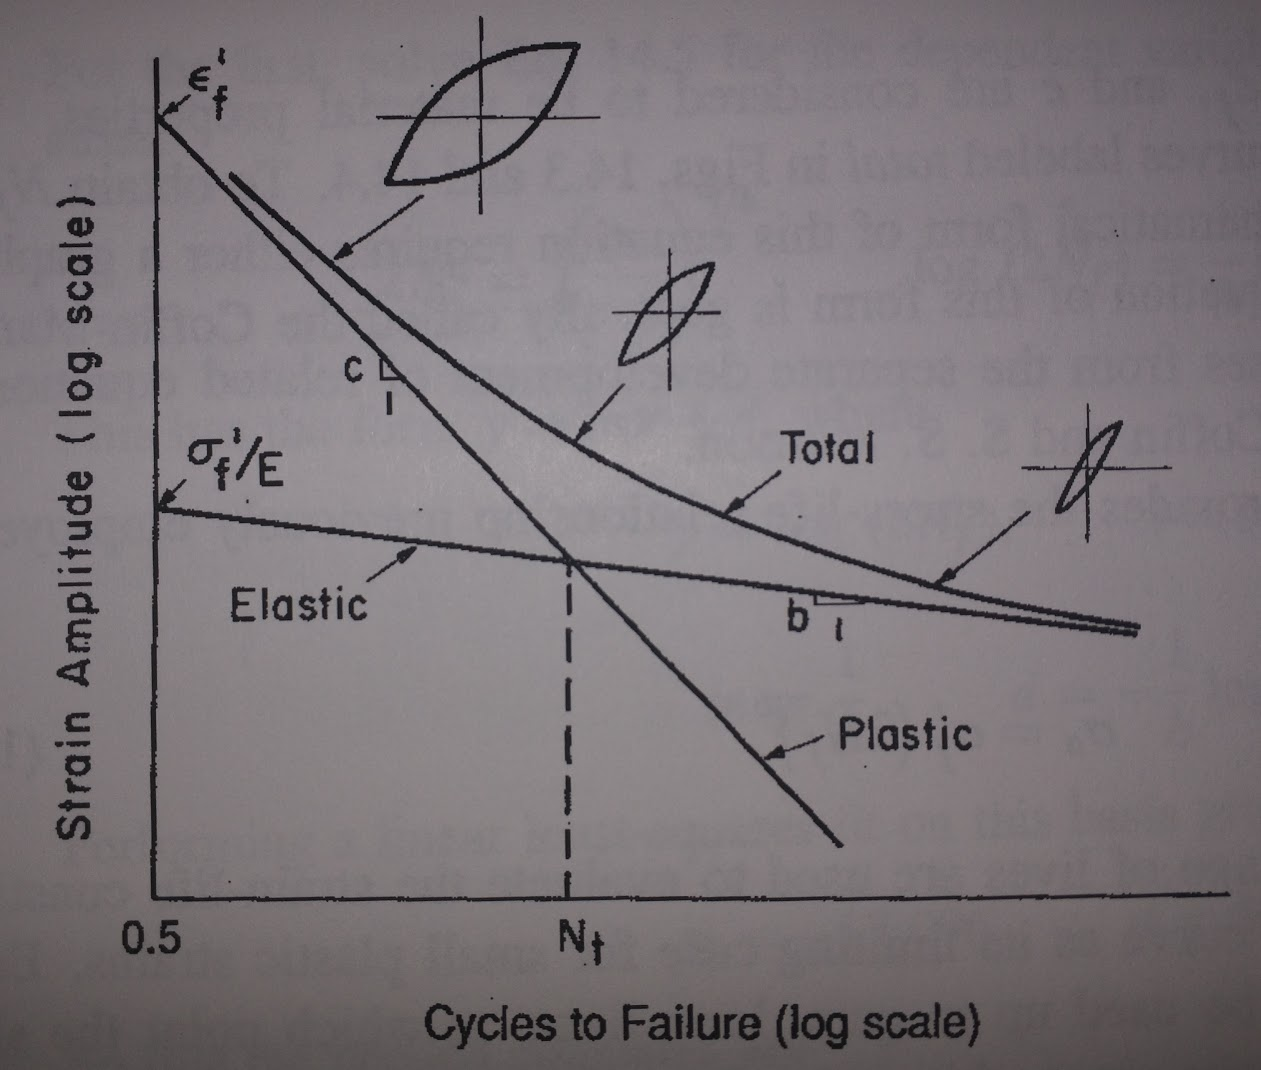
\includegraphics[width=0.7\linewidth]{../Figures/elastic-plastic}
	\label{fig:elastic-plastic}
	\end{figure}
\end{frame}

\begin{frame}{lines}
	\begin{itemize}[<+->]
		\item We notice that the data for elastic and plastic strains are represented by straight lines, in the log-log scale
		\item If we recall the form used for a straight line in log-log plots for S-N curves:
		\item[] \begin{equation}
		\sigma_a = \sigma_f^\prime (2N_f)^b
		\end{equation}
		\item We can convert this to find the elastic component of strain
		\item[] \begin{equation}
		\label{eq:elastic}
		\epsilon_{ea} = \frac{\sigma_f^\prime}{E} (2N_f)^b
		\end{equation}
	\end{itemize}
\end{frame}

\begin{frame}{lines}
	\begin{itemize}[<+->]
		\item We can use the same form with new constants for the plastic component of strain
		\item[]\begin{equation}
		\label{eq:plastic}
		\epsilon_{pa} = \epsilon_f^\prime (2 N_f)^c
		\end{equation}
		\item We can combine \ref{eq:elastic} with \ref{eq:plastic} to find the total strain-life curve
		\item[] \begin{equation}
		\epsilon_a = \frac{\sigma_f^\prime}{E} (2N_f)^b + \epsilon_f^\prime (2 N_f)^c
		\end{equation}
	\end{itemize}
\end{frame}

\begin{frame}{example}
	Data from p. 270	
\end{frame}

\begin{frame}{transition life}
	\begin{itemize}[<+->]
		\item With the strain-based fatigue method we are better equipped to discuss the difference between high and low-cycle fatigue
		\item Low-cycle fatigue is dominated by plastic effects, while high-cycle fatigue has little plasticity
		\item We can find the intersection of the plastic strain and elastic strain lines
		\item This point is $N_t$, the transition fatigue life
		\item[] \begin{equation}
		N_t = \frac{1}{2}\left(\frac{\sigma_f^\prime}{\epsilon_f^\prime}\right)^{\frac{1}{c-b}}
		\end{equation}
	\end{itemize}
\end{frame}

%inconsistencies in constants
\begin{frame}{inconsistencies in constants}
	\begin{itemize}[<+->]
		\item If we consider the equation for the cyclic stress train curve
		\begin{equation}
		\epsilon_a = \frac{\sigma_a}{E} + \left(\frac{\sigma_a}{H^\prime}\right)^{\frac{1}{n^\prime}}
		\end{equation}
		\item We can consider the plastic portion and solve for $\sigma_a$
		\begin{equation}
		\label{eq:stress-life}
		\sigma_a = H^\prime \epsilon_{pa}^{n^\prime}
		\end{equation}
	\end{itemize}
\end{frame}

\begin{frame}{inconsistencies in constants}
	\begin{itemize}[<+->]
		\item We can eliminate $2N_f$ from the plastic strain equation
		\begin{equation}
		\epsilon_{pa} = \epsilon_f^\prime (2N_f)^c
		\end{equation}
		\item By solving the stress-life relationship for $2N_f$
		\begin{equation}
		\sigma_a = \sigma_f^\prime (2N_f)^b
		\end{equation} and substituting that into the plastic strain
		\item We then compare with ~\ref{eq:stress-life} and find
		\begin{subequations}
			\begin{align}
			H^\prime &= \frac{\sigma_f^\prime}{(\epsilon_f^\prime)^{b/c}}\\
			n^\prime &= \frac{b}{c}
			\end{align}
		\end{subequations}
	\end{itemize}
\end{frame}

\begin{frame}{inconsistencies in constants}
	\begin{itemize}[<+->]
		\item However, in practice these constants are fit from different curves
		\item In some cases there can be large inconsistencies in these values
		\item One cause for this is data that do not lie on a straight line in the log-log domain
		\item For ductile materials at short lives, the true stresses and strains may differ significantly from engineering stress and strain
	\end{itemize}
\end{frame}

%trends in metals
\begin{frame}{true fracture strength}
	\begin{itemize}[<+->]
		\item We can consider a tensile test as a fatigue test with $N_f = 0.5$
		\item We would then expect the true fracture strength $\tilde{\sigma}_f \approx \sigma_f^\prime$
		\item And similarly for strain $\tilde{\epsilon}_f \approx \epsilon_f^\prime$
	\end{itemize}
\end{frame}

\begin{frame}{ductile materials}
	\begin{itemize}[<+->]
		\item Since ductile materials experience large strains before failure, we expect relatively large $\epsilon_f^\prime$ and relatively small $\sigma_f^\prime$
		\item This will cause a less steep slope in the plastic strain line
		\item In turn this intersects with the elastic strain line much later, resulting a longer transition life for ductile materials
	\end{itemize}
\end{frame}

\begin{frame}{brittle materials}
	\begin{itemize}[<+->]
		\item Brittle materials exhibit the opposite effect, with relatively low $\epsilon_f^\prime$ and relatively high $\sigma_f^\prime$
		\item This results in a steeper plastic strain line
		\item And shorter transition life 
	\end{itemize}
\end{frame}

\begin{frame}{tough materials}
	\begin{itemize}[<+->]
		\item Tough materials have intermediate values for both $\epsilon_f^\prime$ and $\sigma_f^\prime$
		\item This gives a transition life somewhere between brittle and ductile materials
		\item It is also noteworthy that strain-life for many metals pass through the point $\epsilon_a = 0.01$ and $N_f = 1000$ cycles
	\end{itemize}
\end{frame}

\begin{frame}{typical property ranges}
	\begin{itemize}[<+->]
		\item Most common engineering materials have $-0.8 < c < -0.5$, with most values being very close to $c=-0.6$
		\item The elastic strain slope generally has $b=-0.085$
		\item A "steep" elastic slope is around $b=-0.12$, common in soft metals
		\item While "shallow" slopes are around $b=-0.05$, common for hardened metals
	\end{itemize}
\end{frame}
%creep-fatigue interaction

%surface finish

%mean stress

%multiaxial loading

\end{document}
